\lecture[7]{7. Línulegar nálganir}{lecture-text}
\date{26.~janúar 2015}
\newcounter{mycount}

\begin{document}

\subsection{}
	\maketitle





\subsection{Diffranleiki í einni breytistærð} 

\subsubsection{Skilgreining 7.\arabic{mycount} }
  Látum $f$ vera fall af einni breytistærð og gerum ráð fyrir að $f$ sé
skilgreint á opnu bili sem inniheldur punktinn $a$.  Fallið $f$ er
sagt vera {\em diffranlegt} í punkti $a$ ef markgildið
$$f'(a)=\lim_{h\rightarrow 0}\frac{f(a+h)-f(a)}{h}$$
er til.







\subsection{Diffranleiki í einni breytistærð - önnur lýsing} 

\subsubsection{Skilgreining 7.\arabic{mycount} }\stepcounter{mycount}
Látum $f$ vera fall af einni breytistærð og gerum ráð fyrir að $f$ sé
skilgreint á opnu bili sem inniheldur punktinn $a$.  Fallið $f$ er
sagt vera {\em diffranlegt} í punkti $a$ ef til er tala $m$ þannig að
ef $L(x)=f(a)+m(x-a)$ þá er 
$$\lim_{h\rightarrow 0}\frac{f(a+h)-L(a+h)}{h}=0.$$
(Talan $m$ verður að vera jöfn $f'(a)$.)


\bigskip
Fallið $f$ er 'nálægt' línunni $L$ nálægt punktinum $a$.


\subsection{Diffranleiki} 

\subsubsection{Skilgreining 7.\arabic{mycount}}\stepcounter{mycount}
Fall $f(x,y)$ sem er skilgreint á opinni
skífu umhverfis $(a,b)$ er sagt vera diffranlegt í punktinum $(a,b)$
ef báðar fyrsta stigs hlutafleiður $f$ eru skilgreindar í $(a,b)$ og ef 
$$\lim_{(h,k)\rightarrow (0,0)}
\frac{f(a+h, b+k)-S(a+h,b+k)}{\sqrt{h^2+k^2}}=0$$
þar sem $S(x,y) = f(a,b) + f_1(a,b)(x-a)+f_2(a,b)(y-b)$.

\bigskip
Fallið $f$ er 'nálægt' sléttunni $S$ nálægt punktinum $(a,b)$.


\subsection{Snertiplan}
  Ef $f$ er diffranlegt í $(a,b)$ þá kallast planið $S$ \emph{snertiplan} við graf fallsins.
  \begin{figure}
           \centering
            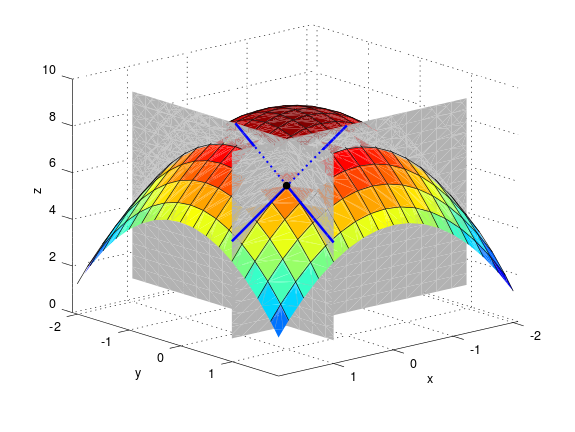
\includegraphics[width=0.6\linewidth]{bothpart.png}
    \end{figure}
    $S(x,y) = f(a,b) + f_1(a,b)(x-a)+f_2(a,b)(y-b)$.



\subsection{Diffranleiki} 

\subsubsection{Setning 7.\arabic{mycount} (Meðalgildissetningin)}\stepcounter{mycount}
Gerum ráð fyrir að fallið $f$
sé samfellt á lokaða bilinu $[a,b]$ og diffranlegt á opna bilinu
$(a,b)$.  Þá er til punktur $c$ á opna bilinu $(a,b)$ þannig að 
$$f(b)-f(a)=f'(c)(b-a).$$





\subsection{Diffranleiki} 

\subsubsection{Setning 7.\arabic{mycount}}\stepcounter{mycount}

Látum  $f(x,y)$ vera fall
sem er skilgreint á opinni 
skífu $\cal D$ með miðju í $(a,b)$ þannig að á þessari skífu eru báðar
fyrsta stigs hlutafleiður $f$ skilgreindar og samfelldar.  Gerum ráð fyrir að $h$
og $k$ séu tölur þannig að $(x+h, y+k)\in{\cal D}$.  Þá eru til tölur
$\theta_1$ og $\theta_2$ á milli 0 og 1 þannig að 
$$f(a+h,b+k)-f(a,b)=hf_1(a+\theta_1h,b+k)+kf_2(a,b+\theta_2k).$$




\subsection{Diffranleiki} 

\subsubsection{Setning 7.\arabic{mycount}}\stepcounter{mycount}
  Látum  $f(x,y)$ vera fall
sem er skilgreint á opinni 
skífu $\cal D$ með miðju í $(a,b)$ þannig að á þessari skífu eru báðar
fyrsta stigs hlutafleiður $f$ skilgreindar og samfelldar. 
Þá er fallið $f$ diffranlegt í $(a,b)$.





\subsection{Diffranleiki} 

\subsubsection{Setning 7.\arabic{mycount}}\stepcounter{mycount}
  Gerum ráð fyrir að $f(x,y)$ sé fall sem er
diffranlegt í punktinum $(a,b)$.  Þá er $f$ samfellt í $(a,b)$.





\subsection{Diffranleiki} 

\subsubsection{Keðjuregla 7.\arabic{mycount}}\stepcounter{mycount}
 Ritum $z=f(x,y)$ þar sem $x=x(s,t)$ og
$y=y(s,t)$.  Gerum ráð fyrir að 

(i) $x(a,b)=p$ og $y(a,b)=q$;

(ii) fyrsta stigs hlutafleiður $x(s,t)$ og $y(s,t)$ eru skilgreindar í
punktinum $(a,b)$;

(iii)  fallið $f$ er diffranlegt í punktinum $(p,q)$.

Þá eru fyrsta stigs hlutafleiður $z$ með tilliti til breytanna $s$ og
$t$ skilgreindar í punktinum $(a,b)$ og um þær gildir að 
$$\frac{\partial z}{\partial s}=
\frac{\partial z}{\partial x}\frac{\partial x}{\partial s}
+\frac{\partial z}{\partial y}\frac{\partial y}{\partial s}$$
og
$$\frac{\partial z}{\partial t}=
\frac{\partial z}{\partial x}\frac{\partial x}{\partial t}
+\frac{\partial z}{\partial y}\frac{\partial y}{\partial t}.$$




\subsection{Diffur} 

\subsubsection{Skilgreining 7.\arabic{mycount}}\stepcounter{mycount}
  Ritum $z=f(x_1, x_2, \ldots, x_n)$.  {\em
  Diffrið} af $z$ er skilgreint sem 
$$dz=df=\frac{\partial z}{\partial x_1}dx_1
+\frac{\partial z}{\partial x_2}dx_2
+\cdots+\frac{\partial z}{\partial x_n}dx_n.$$
Diffrið er nálgun á 
$$\Delta f=f(x_1+dx_1, x_2+dx_2,\ldots,
x_n+dx_n)-f(x_1,x_2,\ldots,x_n).$$




\subsection{Varpanir $\Rn\rightarrow\Rm$} 
\subsubsection{Táknmál 7.\arabic{mycount}}\stepcounter{mycount}
Látum $\fv:\Rn\rightarrow\Rm$ tákna vörpun.
Ritum $\fv=(f_1,\ldots,f_m)$ þar sem hvert $f_i$ er fall
$\Rn\rightarrow\R$.  Fyrir punkt í $\Rn$ ritum við
$\xv=(x_1,x_2,\ldots,x_n)$.  Síðan ritum við $\yv=\fv(\xv)$ þar sem 
$\yv=(y_1,y_2,\ldots,y_m)$ og 
\Wider{$$y_1=f_1(x_1,x_2,\ldots,x_n),y_2=f_2(x_1,x_2,\ldots,x_n),
\ldots, y_m=f_m(x_1,x_2,\ldots,x_n).$$}




\subsection{Jacobi-fylki} 
 \subsubsection{Skilgreining 7.\arabic{mycount}}\stepcounter{mycount}
 Notum táknmálið úr 7.8.
Ef allar hlutafleiðurnar $\partial
y_i/\partial x_j$ eru skilgreindar í punktinum $\xv$ þá skilgreinum
við {\em Jacobi-fylki} $f$ í punktinum $\xv$ sem $m\times n$ fylkið
$$D\fv(\xv)=\begin{bmatrix}
\frac{\partial y_1}{\partial x_1}&\frac{\partial y_1}{\partial x_2}&
\cdots&\frac{\partial y_1}{\partial x_n}\\
\frac{\partial y_2}{\partial x_1}&\frac{\partial y_2}{\partial x_2}&
\cdots&\frac{\partial y_2}{\partial x_n}\\
\vdots&\vdots&\ddots&\vdots\\
\frac{\partial y_m}{\partial x_1}&\frac{\partial y_m}{\partial x_2}&
\cdots&\frac{\partial y_m}{\partial x_n}
\end{bmatrix}$$



\subsection{Diffranleiki varpana $\Rn\rightarrow\Rm$} 
 \subsubsection{Skilgreining 7.\arabic{mycount}}\stepcounter{mycount}
 Notum táknmálið úr 7.8 og 7.9. Látum $\av=(a_1, a_2, \ldots, a_n)$ vera fastan punkt í $\Rn$ og ritum 
$\hv=(h_1,h_2,\ldots,h_n)$.  Vörpunin $\fv$ er
sögð diffranleg í punktinum $\av$ ef
$$\lim_{\hv\rightarrow
  \ov}\frac{|\fv(\av+\hv)-\fv(\av)-D\fv(\av)\hv|}{|\hv|}=0.$$ 

\bigskip
Vörpunin $f$ er 'nálægt' línulegu vörpuninni $D\fv$ nálægt punktinum $\av$.

\bigskip
Línulega vörpunin $D\fv$ kallast afleiða $\fv$.



\subsection{Keðjureglan} 
 \subsubsection{Setning 7.\arabic{mycount}}\stepcounter{mycount}
Látum $\fv:\Rn\rightarrow \Rm$ og 
$\gv:\Rm\rightarrow \Rk$ vera varpanir.  Gerum ráð fyrir að vörpunin
$\fv$ sé diffranleg í punkti $\xv$ og vörpunin $\gv$ sé diffranleg í
punktinum $\yv=\fv(\xv)$.  Þá er samskeytta vörpunin
$\gv\circ\fv:\Rn\rightarrow\Rk$ diffranleg í $\xv$ og 
$$D(\gv\circ\fv)(\xv)=D\gv(\fv(\xv))D\fv(\xv).$$







\end{document}